\documentclass{ethz_report}
\usepackage{listings}
\usepackage{color}
\usepackage{caption}
\usepackage{subcaption}


\definecolor{codegreen}{rgb}{0,0.6,0}
\definecolor{codegray}{rgb}{0.5,0.5,0.5}
\definecolor{codepurple}{rgb}{0.58,0,0.82}
\definecolor{backcolour}{rgb}{1,1,1}

\lstdefinestyle{mystyle}{
    backgroundcolor=\color{backcolour},
    commentstyle=\color{codegreen},
    keywordstyle=\color{magenta},
    numberstyle=\tiny\color{codegray},
    stringstyle=\color{codepurple},
    basicstyle=\ttfamily,
    breakatwhitespace=false,
    breaklines=true,
    captionpos=b,
    keepspaces=true,
    numbers=left,
    numbersep=5pt,
    showspaces=false,
    showstringspaces=false,
    showtabs=false,
    tabsize=4,
    frame=lines
}
\lstset{style=mystyle}

\title{Exercise 2 - Camera Calibration}
\subject{Computer Vision}
\author{Alberto Montes}
\email{malberto@student.ethz.ch}
\date{\today}

\begin{document}
\maketitle

\section*{Data Normalization}

The first step after capturing the points from the taken images is to transform the coordinates to homogeneous vectors.

\lstinputlisting[language=MATLAB, caption=Transform to Homogeneous Vectors, firstline=3, lastline=6]{../code/runDLT.m}

The next one has been implement the data normalization, which consist in substracting the centroid and scale all points to have mean distance to the centroid equivalent to $\sqrt{2}$ and $\sqrt{3}$ for 2D and 3D points respectively. Finding the centroid and the scale factor, it is only necessary to construct the transformation matrix as it is done in Listing~\ref{lst:normalization}.

\lstinputlisting[language=MATLAB, caption=normalization.m, label={lst:normalization}]{../code/normalization.m}

\section*{Direct Linear Transform}

The DLT consist in different steps, starting with the previous presented one, data normalization.
In Listing~\ref{lst:process_dlt} there is the differents steps to go through to use the DLT method.

\lstinputlisting[language=MATLAB, caption=runDLT.m, firstline=8, lastline=17, label={lst:process_dlt}]{../code/runDLT.m}

The next step consists into find the matrix transformation between the 3D and 2D points. To find this matrix is mandatory to use the normalized points to find the normalized matrix to then denormalize the camera matrix found. In Listing~\ref{lst:dlt} is the code use to compute the camera matrix.

\lstinputlisting[language=MATLAB, caption=dlt.m, label={lst:dlt}]{../code/dlt.m}

Once you have computed this matrix, it can be decomposed into the intrinsic matrix, the camera orientation rotation matrix and the camera center. To do this is used the code in Listing~\ref{lst:decompose}.

\lstinputlisting[language=MATLAB, caption=decompose.m, label={lst:decompose}]{../code/decompose.m}

Finally, the reprojected points have been computed from the computed transformation matrix as well as the error of this reprojection. When computing the reprojected points it has to take into account that the points need to normalize such that the last component is 1 and fits the homogeneus coordinates.

\lstinputlisting[language=MATLAB, caption=Computing reprojected points (runDLT.m), firstline=18, lastline=22]{../code/runDLT.m}

The resulting mean error of the DLT method to the test image has been: $37.606$.
The reprojected points computed with the Direct Linear Transform can be found on Figure~\ref{fig:results_dlt}.

\begin{figure}[H]
\centering
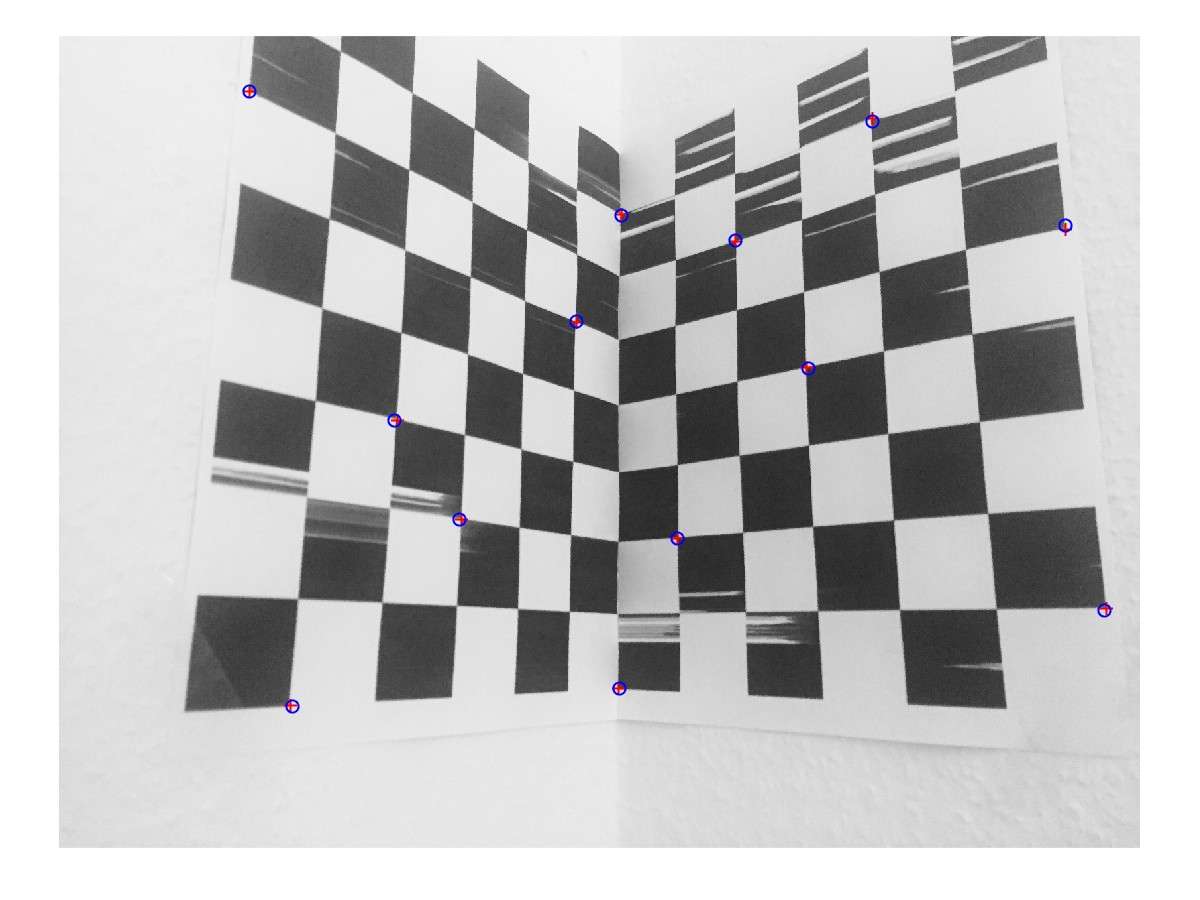
\includegraphics[width=.9\linewidth]{images/DLT_reprojected}
\caption{Reprojected points using the DLT method}
\label{fig:results_dlt}
\end{figure}

\section*{Gold Standard algorithm}

The Gold Standard algorithm works basically the same as the DLT method, but in addition, try to minimize the error caused by the camera matrix, trying to find its optimal values.

\lstinputlisting[language=MATLAB, caption=runGoldStandard.m, firstline=7, lastline=23, label={lst:process_gold}]{../code/runGoldStandard.m}

It basically starts with the same steps as the DLT, even computing the camera matrix with this method, and once it has an initial value for the matrix, tries to find the optimal values for the matrices that minimizes the sum squared error.
To find the optimal values, it has been defined the function in Listing~\ref{lst:fmin} which computes the sum of squared error of the reprojected points given a camera matrix, and iteratively is found the optimal values.

\lstinputlisting[language=MATLAB, caption=fminGoldStandard.m, label={lst:fmin}]{../code/fminGoldStandard.m}

Using the search of the optimal values for the camera matrix which minimizes the error of the reprojected points, I have arrived into a decrease of the error to $36.344$.
The reprojected points are plot in Figure~\ref{fig:results_gold}.

\begin{figure}[H]
\centering
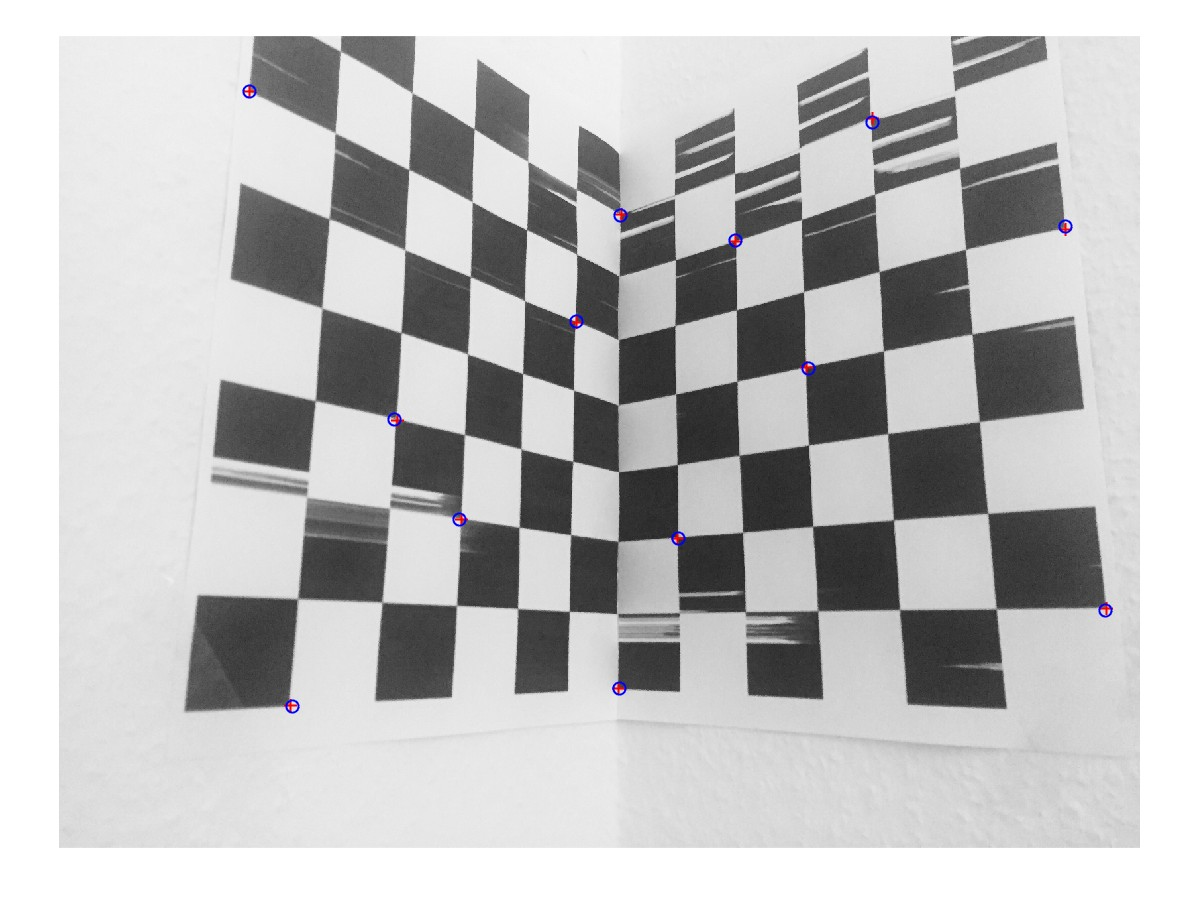
\includegraphics[width=.9\linewidth]{images/GoldStd_reprojected}
\caption{Reprojected points using the Gold Standard Algorithm}
\label{fig:results_gold}
\end{figure}

Comparison between the DLT method and the Gold Standard algorithm can be found in Figure~\ref{fig:results_comparison}. The results are very similar, no distinguishable at the image but the error shows that the Gold Standard algorithm works better than the Direct Linear Transform.

\begin{figure}[H]
\centering
\begin{subfigure}[b]{.5\textwidth}
  \centering
  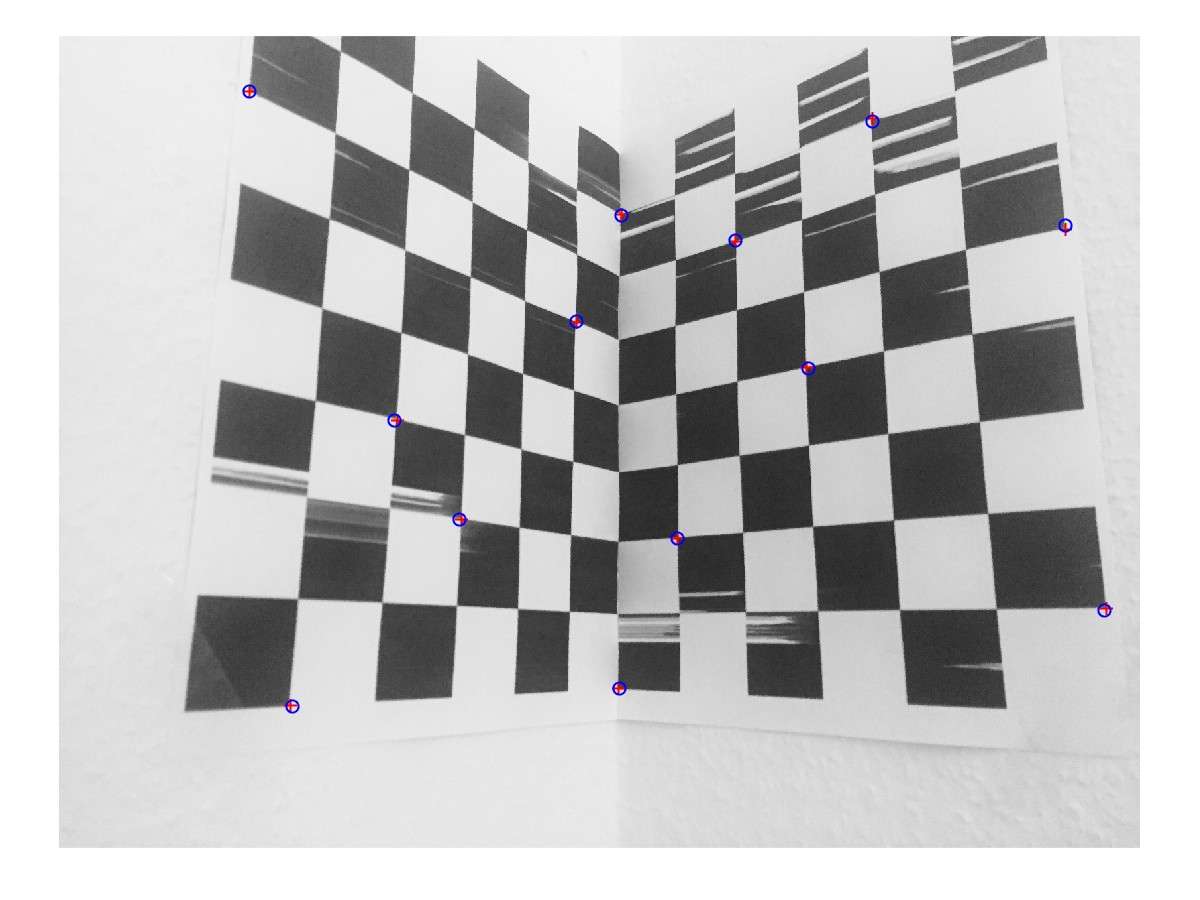
\includegraphics[width=1\linewidth]{images/DLT_reprojected}
  \caption{Direct Linear Transform}
\end{subfigure}%
\begin{subfigure}[b]{.5\textwidth}
  \centering
  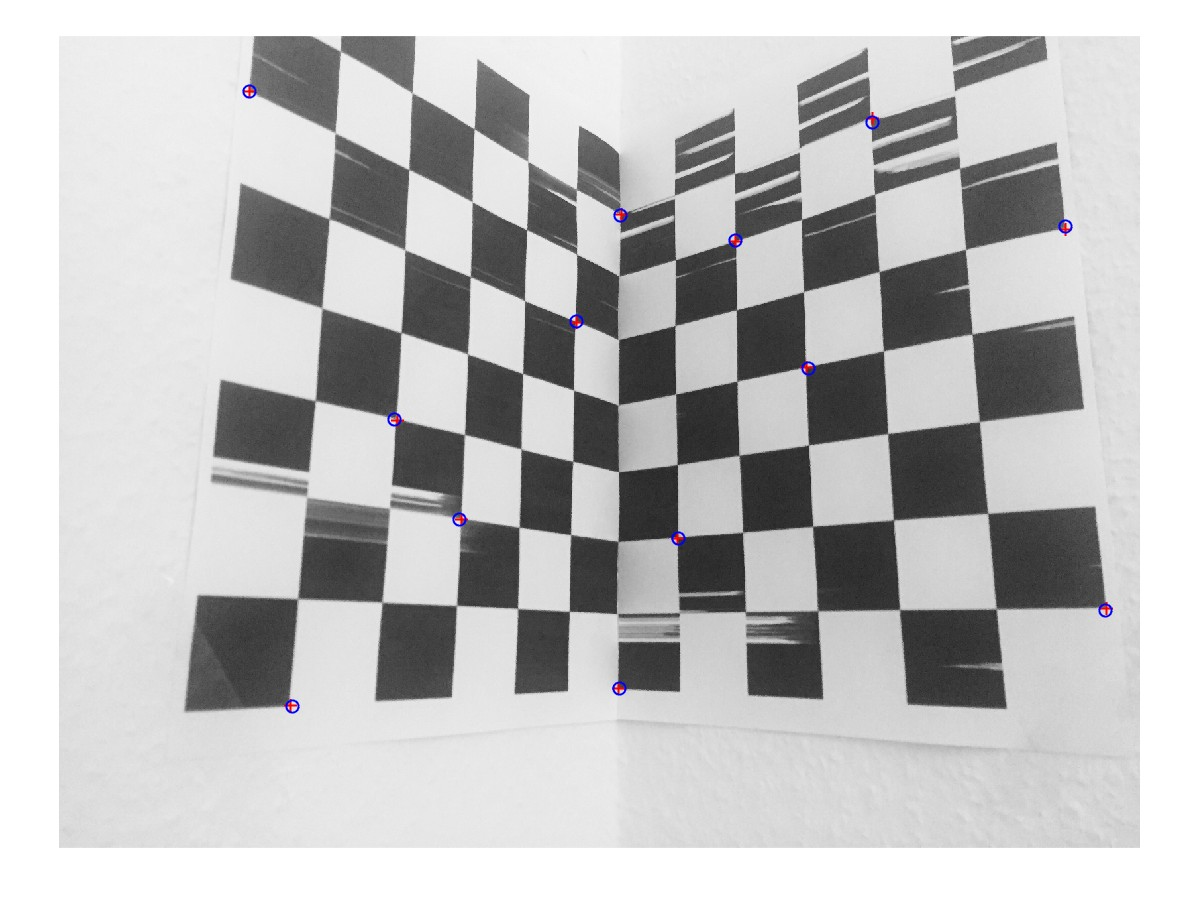
\includegraphics[width=1\linewidth]{images/GoldStd_reprojected}
  \caption{Gold Standard Algorithm}
\end{subfigure}
\caption{Comparing results}
\label{fig:results_comparison}
\end{figure}

\section*{Bouget's Calibration Toolbox}


\end{document}
